\documentclass{thesis}
\usepackage[utf8]{inputenc} %
\usepackage[T5]{fontenc} % Font Vietnamese
\usepackage{graphicx} % Figure
\usepackage{float} % Set position figure or table
\usepackage{mathptmx} % select font Times New Roman
\usepackage{geometry} % Set parameters paper
\usepackage{xcolor}
\usepackage[fontsize=13pt]{scrextend} % set font size = 13pt
\usepackage{indentfirst} % Indent first line
% \usepackage{microtype}
\usepackage[protrusion=false]{microtype}
\usepackage{titling}
\usepackage{multicol}

%% START DOCUMENT
\begin{document}

% CREATE COVER PAGE

\begin{center}
  \vspace{12pt} % line spacing
  \textbf{\fontsize{15pt}{0pt} \selectfont{} ĐẠI HỌC BÁCH KHOA HÀ NỘI }
  \vspace{0.5cm}

  % INSERT LOGO
  \begin{figure}[H]
    \centering
    
\includegraphics[width=2cm,height=3cm]{logoBK.png}
  \end{figure}

  % THESIS TYPE
  \vspace{48pt}
  \fontsize{25pt}{0pt}{\fontfamily{qag}\selectfont{} \textbf{BÁO CÁO BÀI TẬP
  LỚN MÔN HỌC: HỆ THỐNG QUẢN LÝ TOÀ NHÀ THÔNG MINH}}
  \vspace{24pt}

  % THESIS TITTLE
  \fontsize{17pt}{0pt}{\fontfamily{qag}\selectfont{} \textbf {ĐỀ TÀI: NĂNG
  LƯỢNG MẶT TRỜI\\TRONG TOÀ NHÀ THÔNG MINH}}
  \vspace{18pt}

  % % NAME
  % \fontsize{14pt}{0pt}\selectfont{} \textbf{ĐINH HOÀNG SƠN}
  % \vspace{3pt}
  %
  % % EMAIL
  % \fontsize{14pt}{0pt}\selectfont{} son.dh241853e@sis.hust.edu.vn
  % \vspace{12pt} % line spacing

  \begin{center}
    \fontsize{14pt}{18pt}\selectfont
    \begin{tabular}{|l|l|}
      \hline
      \textbf{Tên sinh viên} & \textbf{Mã số sinh viên} \\ \hline
      ĐINH HOÀNG SƠN    & 2241853E \\ \hline
      LÊ QUÝ DƯƠNG      & 20241714E \\ \hline
      NGUYỄN QUANG MINH & 20241808E \\ \hline
      VŨ MINH PHƯƠNG    & 20250954E \\ \hline
    \end{tabular}
  \end{center}

  % % MAJOR
  % \fontsize{14pt}{0pt}\selectfont{} \textbf{Ngành Kỹ thuật Điều khiển
  % và Tự động hóa}
\end{center}
\vspace{48pt}

% INFORMATION: SUPERVISOR NAME, STUDENT NAME,...
\begin{table}[H]
  \centering
  \begin{tabular}{l l c}
    \textbf{Giảng viên hướng dẫn:}    &  TS. Nguyễn Hoàng Nam \vspace{6pt} &  \\
    &\vspace{3pt} & \fontsize{10pt}{0pt}\selectfont{} Chữ ký của GVHD \\
    \textbf{Mã học phần:} & EE4269 \vspace{3pt}\\
    \textbf{Mã lớp:} & 173738 \vspace{3pt}\\
    \textbf{Khoa:} & Tự động hóa \vspace{3pt}\\
    \textbf{Trường:} & Điện - Điện tử
  \end{tabular}
\end{table}

% TIME
\begin{center}
  \vspace{48pt}
  \fontsize{14pt}{0pt}\selectfont{} \textbf{Hà Nội, 06/2027}
\end{center}

% CREATE A NEW PAGE AND REMOVE PAGE NUMBER
\thispagestyle{empty}
\newpage
%     \clearpage
%            \thispagestyle{empty}
%              \cleardoublepage

% THESIS TASK

\thispagestyle{empty}
\newpage
%        \clearpage
%           \thispagestyle{empty}
%               \cleardoublepage

% THANKS
\section*{LỜI CẢM ƠN}
\thispagestyle{empty}
Đây là mục tùy chọn, nên viết phần cảm ơn ngắn gọn, tránh dùng các từ sáo rỗng.

\vspace{6pt}
\hspace{7cm}Hà Nội, ngày 05 tháng 09 năm 2027

\hspace{8.6cm} Sinh viên thực hiện      % command '\hspace' used to line indents

\vspace{2cm}
\hspace{9.25cm}\textbf{Đinh Hoàng Sơn} % change name

\newpage % create a new page
%    \thispagestyle{empty}
%        \clearpage
%            \thispagestyle{empty}
%              \cleardoublepage

% SUMMARY PART
\section*{TÓM TẮT ĐỒ ÁN}
\thispagestyle{empty}
Tóm tắt nội dung của đồ án tốt nghiệp trong khoảng tối đa 300 chữ.
Phần tóm tắt cần nêu được các ý: vấn đề cần thực hiện; phương pháp
thực hiện; công cụ sử dụng (phần mềm, phần cứng…); kết quả của đồ án
có phù hợp với các vấn đề đã đặt ra hay không; tính thực tế của đồ
án, định hướng phát triển mở rộng của đồ án (nếu có); các kiến thức
và kỹ năng mà sinh viên đã đạt được.

\thispagestyle{empty}
\cleardoublepage

% CONTENT
\tableofcontents
\thispagestyle{empty}
\newpage
%           \thispagestyle{empty}
%              \cleardoublepage

% LIST OF SYMBOLS AND ABBREVIATIONS
\pagenumbering{roman}   % Roman numbering: i, ii, iii, iv,...
\section*{DANH MỤC KÝ HIỆU VÀ CHỮ VIẾT TẮT}
\phantomsection \addcontentsline{toc}{section}{\numberline{} DANH MỤC
KÝ HIỆU VÀ CHỮ VIẾT TẮT}

% Create table
\begin{tabular}{ l l }
  \hspace{1cm} BDA & \hspace{2cm} Bidirection Amplifier \\
  \hspace{1cm} CAM & \hspace{2cm} Common Area Maintenance \\
  \hspace{1cm} CLEC & \hspace{2cm} Competitive Local Exchange Carrier \\
  \hspace{1cm} DAS & \hspace{2cm} Distributed Antenna System \\
  \hspace{1cm} FCC & \hspace{2cm} Federal Communications Commission \\
  \hspace{1cm} NFPA & \hspace{2cm} National Fire Protection Association \\
  \hspace{1cm} PSAP & \hspace{2cm} Public Safety Answering Points \\
  \hspace{1cm} RF & \hspace{2cm} Radio Frequency \\
  \hspace{1cm} SLA & \hspace{2cm} Service Level Agreements \\
  \hspace{1cm} DC & \hspace{2cm} Direct Current \\
  \hspace{1cm} AC & \hspace{2cm} Alternating Current \\
  \hspace{1cm} IT & \hspace{2cm} Information Technology \\
  \hspace{1cm} POE & \hspace{2cm} Power Over Ethernet \\
  \hspace{1cm} IEEE & \hspace{2cm} Institute of Electrical and
  Electronics Engineers \\
  \hspace{1cm} IP & \hspace{2cm} Internet Protocol \\
  \hspace{1cm} VoIP & \hspace{2cm} Voice-over IP \\

\end{tabular}
\newpage

% LIST OF FIGURES
{\let\oldnumberline\numberline
  \renewcommand{\numberline}{Hình~\oldnumberline}
\listoffigures}
\phantomsection\addcontentsline{toc}{section}{\numberline{} DANH MỤC HÌNH VẼ}
\newpage

% LIST OF TABLES
{\let\oldnumberline\numberline
  \renewcommand{\numberline}{Bảng~\oldnumberline}
\listoftables}
\phantomsection\addcontentsline{toc}{section}{\numberline{} DANH MỤC BẢNG BIỂU}
\newpage

%% --------------------------------------------------%%
%------------CHAPTER 1---------------------------%
%%-----------------------------------------------------%

\pagenumbering{arabic} % numbering: 1,2,3,...
\section*{CHƯƠNG 11. HỆ THỐNG ĂNG-TEN PHÂN TÁN (DAS)}
\phantomsection
\addcontentsline{toc}{section}{\numberline{}CHƯƠNG 11. HỆ THỐNG
ĂNG-TEN PHÂN TÁN (DAS)} % Reference to content

\setcounter{section}{11}
\setcounter{subsection}{0}
\setcounter{figure}{0}
\setcounter{table}{0}
%%--------------------------------------------------------

Điện thoại di động đã trở thành một phần quen thuộc của đời sống hiện
đại, phục vụ công việc, giải trí và giao tiếp hằng ngày. Theo Liên
minh Viễn thông Quốc tế (ITU), năm 2013 thế giới có khoảng 6,8 tỷ
thuê bao di động, gần bằng dân số khoảng 7 tỷ người, tương đương 96
thuê bao trên 100 người. Tuy nhiên, số thuê bao không phản ánh chính
xác số người sử dụng vì một người có thể sở hữu nhiều thiết bị hoặc
đăng ký nhiều thuê bao. Tại các quốc gia phát triển, tỷ lệ này thường
vượt 100\%; ngay cả ở các nước đang phát triển và có thu nhập thấp, tỷ
lệ thuê bao cũng đạt khoảng 90\%. Riêng tại châu Phi, cứ 100 người
chỉ có 1,4 thuê bao điện thoại cố định nhưng có tới 63,5 thuê bao di động.
Nhiều nghiên cứu đã khảo sát thói quen sử dụng và mức độ phụ thuộc
của con người vào điện thoại thông minh. Một khảo sát với 2.000 người
tham gia cho thấy người dùng thường bắt đầu sử dụng điện thoại vào
khoảng 7 giờ 31 phút sáng; nhiều người kiểm tra email cá nhân và
Facebook ngay sau khi thức dậy. Khoảng 40\% số người được hỏi cho biết
họ cảm thấy bất tiện hoặc mất kết nối khi không mang theo điện
thoại. Một nghiên cứu khác ghi nhận người dùng điện thoại thông
minh kiểm tra thiết bị trung bình khoảng 150 lần mỗi ngày.

Khi tỷ lệ thuê bao di động đạt khoảng 90-100\% và con người dành tới
80-90\% thời gian ở trong nhà, chất lượng phủ sóng bên trong công
trình trở thành một yêu cầu quan trọng. Khoảng 80\% cuộc gọi thoại
và 90\% lưu lượng dữ liệu di động phát sinh trong nhà. Tuy nhiên,
tín hiệu tại nhiều công trình vẫn yếu hoặc không ổn định, làm gián
đoạn liên lạc và gây rớt cuộc gọi.

Khả năng thu sóng trong nhà phụ thuộc vào quy mô, chiều cao, mật độ
người sử dụng và vật liệu xây dựng của công trình. Tín hiệu thường
suy giảm tại các tòa nhà cao tầng, nơi tập trung đông người hoặc công
trình sử dụng nhiều thép, nhôm, gạch và bê tông cốt thép. Bên cạnh
các vật liệu kết cấu, loại kính sử dụng cho mặt ngoài công trình cũng
có thể ảnh hưởng đến khả năng truyền sóng. Điển hình là kính Low-E,
loại kính được thiết kế để hạn chế tia tử ngoại và tia hồng ngoại
truyền qua, qua đó giảm lượng nhiệt đi vào tòa nhà và tiết kiệm năng
lượng. Tuy nhiên, lớp phủ trên kính cũng phản xạ một phần sóng vô
tuyến, khiến tín hiệu di động truyền vào bên trong công trình bị suy giảm.

Chất lượng dịch vụ không dây còn giảm khi mạng không đủ dung lượng
đáp ứng nhu cầu sử dụng. Tình trạng này thường xuất hiện tại những
nơi tập trung đông người hoặc phát sinh lưu lượng dữ liệu lớn, chẳng
hạn sân vận động, trung tâm hội nghị, tòa nhà văn phòng, trường đại
học, bệnh viện, cơ sở sản xuất, khách sạn, chung cư cao tầng, cơ quan
hành chính và hệ thống đường sắt hoặc tàu điện ngầm.

Vùng phủ sóng di động trong tòa nhà thường gặp hai vấn đề: tín hiệu
từ trạm phát sóng gần nhất quá yếu hoặc dung lượng mạng không đủ. Do
nguyên nhân khác nhau, mỗi vấn đề cần một giải pháp xử lý riêng.

Khi tín hiệu yếu, giải pháp phổ biến là sử dụng bộ lặp để thu và
khuếch đại tín hiệu từ trạm phát sóng gần nhất. Một ăng-ten ngoài
trời được lắp trên công trình và hướng về phía trạm phát để thu tín
hiệu. Tín hiệu sau đó truyền qua cáp tới bộ khuếch đại hai chiều
(BDA). Thiết bị này khuếch đại tín hiệu theo cả hai hướng: từ trạm
phát tới thiết bị di động và từ thiết bị di động trở lại trạm gốc.
Nhờ đó, các thiết bị bên trong công trình có thể duy trì liên lạc ổn
định hơn với mạng di động bên ngoài.

\begin{figure}[!ht]
  \centering
  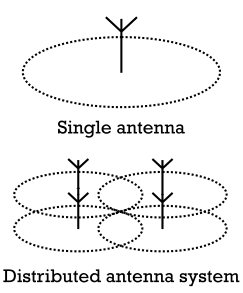
\includegraphics{images/h11.1.png} % Link to figure
  \caption{Hệ thống ăng-ten phân tán (DAS)} % figure name
  \label{images/h11.1.png}  % cross-reference for figure
\end{figure}

Khi nguyên nhân chính là thiếu dung lượng, giải pháp thường được sử
dụng là bố trí nhiều ăng-ten nhỏ trong tòa nhà. Hệ thống chủ động này
được gọi là hệ thống ăng-ten phân tán (Distributed Antenna System -
DAS). DAS gồm các bộ khuếch đại và ăng-ten được phân bố trong công
trình, liên kết bằng cáp đồng hoặc cáp quang về một đầu mối trung
tâm. Hệ thống cung cấp dịch vụ thoại và dữ liệu không dây trong một
công trình hoặc khu vực xác định.
Đầu cuối trung tâm của DAS cho phép nhiều nhà mạng kết nối thiết bị
vô tuyến hoạt động trên các dải tần khác nhau. Với mô hình DAS dùng
chung cho nhiều nhà mạng (neutral-host DAS), nhiều nhà mạng có thể
khai thác chung một hệ thống hạ tầng. Tín hiệu của từng nhà mạng được
phân phối tới các ăng-ten nhỏ để phủ sóng theo từng khu vực hoặc từng
tầng của tòa nhà. DAS có thể được triển khai cả trong nhà và ngoài
trời. Đối với hệ thống ngoài trời, cơ quan quản lý tiện ích công cộng
tại một số bang của Hoa Kỳ yêu cầu đơn vị quản lý hạ tầng tạo điều
kiện lắp đặt DAS trong hành lang kỹ thuật công cộng

\subsection{Mô hình kinh doanh DAS}

Ban đầu, các nhà mạng triển khai DAS để mở rộng vùng phủ sóng vào bên
trong tòa nhà. Nhà mạng đầu tư, lắp đặt và bảo trì hệ thống với kỳ
vọng tăng doanh thu từ dịch vụ. Sau đó, họ nhận thấy hạ tầng này có
thể được khai thác hiệu quả hơn bằng cách cho các nhà mạng khác cùng
sử dụng. Từ đó, mô hình neutral-host DAS được hình thành.

DAS mang lại lợi ích cho cả chủ sở hữu công trình và nhà mạng. Vùng
phủ sóng được cải thiện giúp người thuê và người sử dụng liên lạc ổn
định hơn, đồng thời giảm số khiếu nại và yêu cầu hỗ trợ. Đối với chủ
sở hữu, khả năng kết nối tốt giúp công trình hấp dẫn hơn với khách
thuê và hỗ trợ các dịch vụ khẩn cấp. Đối với nhà mạng, lưu lượng
thoại và dữ liệu tăng có thể tạo thêm doanh thu.

\begin{figure}[!ht]
  \centering
  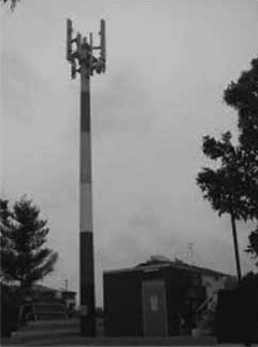
\includegraphics{images/h11.2.png} % Link to figure
  \caption{Trạm phát sóng di động}
  \label{images/h11.2.png}
\end{figure}

\begin{figure}[!ht]
  \centering
  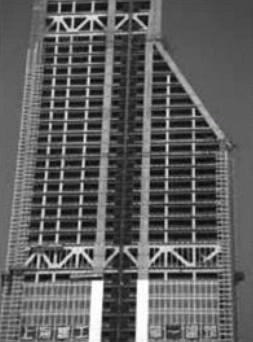
\includegraphics{images/h11.3.png} % Link to figure
  \caption{Nhiều ăng-ten trong một tòa nhà quy mô lớn}
  \label{images/h11.3.png}
\end{figure}

Theo dự báo của iGR Research tại thời điểm tài liệu được công bố, số
lượng hệ thống DAS lắp đặt có thể tăng 300\% vào năm 2017. Sự tăng
trưởng này xuất phát từ nhu cầu kết nối ổn định, yêu cầu băng thông
cao hơn và kỳ vọng ngày càng lớn về chất lượng dịch vụ. Một hệ thống
DAS điển hình khi đó có chi phí khoảng 5-10 triệu đô la Mỹ. Doanh thu
của thị trường DAS toàn cầu đạt 2 tỷ đô la Mỹ vào năm 2013.

DAS có thể được đầu tư và vận hành theo ba mô hình. Trong mô hình thứ
nhất, chủ sở hữu tòa nhà sở hữu hệ thống và chịu trách nhiệm cung cấp
dịch vụ, bảo trì và nâng cấp. Ở mô hình thứ hai, một đơn vị thứ ba
đầu tư mạng trung lập dùng chung cho nhiều nhà mạng, đồng thời trực
tiếp vận hành, quản lý và giám sát hệ thống. Nhờ đó, chủ sở hữu tòa
nhà không phải tự đầu tư vào DAS. Trong mô hình thứ ba, chủ sở hữu và
đơn vị thứ ba cùng góp vốn; đơn vị thứ ba sở hữu mạng và phụ trách
việc bảo trì, cung cấp dịch vụ cũng như làm việc với các nhà mạng.

Nhìn chung, các nhà mạng ít sẵn sàng tài trợ DAS cho tòa nhà văn
phòng hoặc trung tâm thương mại thông thường. Họ thường ưu tiên sân
bay, sân vận động và khuôn viên doanh nghiệp lớn, nơi có mức độ nhận
diện cao và khả năng thu hồi vốn tốt hơn. Do chi phí đầu tư và vận
hành DAS khá lớn, hiệu quả tài chính tại các công trình nhỏ thường
khó được chứng minh. Vì vậy, nhà mạng có thể trực tiếp lắp đặt và vận
hành hệ thống tại sân vận động hoặc sân bay nhưng ít khi áp dụng cách
này cho tòa nhà quy mô nhỏ.

Bên cạnh ba mô hình sở hữu và vận hành nêu trên, các tòa nhà lớn có
thể áp dụng một phương án tài chính riêng khi có một đơn vị sử dụng
chính. Đơn vị này thường đồng thời là chủ sở hữu công trình, sử dụng
phần lớn diện tích và cho các tổ chức khác thuê phần còn lại. Nhà
mạng đang phục vụ đơn vị sử dụng chính có thể triển khai hạ tầng
trong tòa nhà, sau đó cung cấp dịch vụ cho những khách thuê khác để
tăng doanh thu. Chủ sở hữu có thể phân bổ chi phí vận hành và bảo trì
hệ thống cho người thuê thông qua tiền thuê bổ sung, phí bảo trì khu
vực chung (Common Area Maintenance - CAM) hoặc phí tiện ích. Các
khoản phí này có thể bao gồm
chi phí cho hệ thống thông tin liên lạc và thiết bị dùng chung.

Nếu đơn vị cung cấp DAS đầu tư hạ tầng và bán lại dịch vụ không dây
cho tòa nhà như một tiện ích, chi phí này có thể được tính vào phí
tiện ích của người thuê. Khi đó, đơn vị cung cấp DAS nên hoạt động
với tư cách nhà cung cấp viễn thông nội hạt cạnh tranh có giấy phép
(Competitive Local Exchange Carrier - CLEC). Chủ sở hữu và đơn vị DAS
sẽ ký thỏa thuận dài hạn, trong đó
quy định quyền sử dụng không gian kỹ thuật, tuyến cáp và vị trí lắp
đặt thiết bị trong công trình. Theo phương án này, đơn vị DAS có
nguồn thu để hoàn vốn; chủ sở hữu không phải tự đầu tư toàn bộ hệ
thống; còn người thuê được sử dụng dịch vụ không dây ổn định hơn.

% Bảng so sánh của Dương

Các bên kinh doanh cần xác định rõ (a) đơn vị sở hữu mạng, (b) nguồn
vốn đầu tư, (c) thỏa thuận với từng nhà mạng và thỏa thuận mức dịch
vụ (SLA) của DAS. SLA quy định phạm vi dịch vụ, yêu cầu chất lượng,
trách nhiệm của các bên và thời hạn đạt mức hiệu năng đã cam kết. Kế
hoạch vận hành và bảo trì cũng phải tính đến việc cải tạo hoặc thay
đổi không gian trong tòa nhà vì những thay đổi này có thể ảnh hưởng
đến hiệu năng của hệ thống ăng-ten. Ngoài ra, sự phát triển của công
nghệ di động, chẳng hạn quá trình chuyển từ 3G sang 4G tại thời điểm
tài liệu được viết, cũng làm phát sinh nhu cầu nâng cấp và điều chỉnh DAS

Một số công trình đã triển khai DAS trong thực tế như sau:

\begin{itemize}
  \item Merchandise Mart, Chicago. Khi khánh thành năm 1930,
    Merchandise Mart là tòa nhà lớn nhất thế giới, với diện tích
    khoảng 4 triệu ft². Hiện nay, công trình sử dụng DAS trung lập
    dùng chung, cho phép nhiều nhà mạng kết nối thiết bị vô tuyến và
    phát tín hiệu trên cùng một hạ tầng. Đầu cuối trung tâm của hệ
    thống được bố trí trong không gian rộng 2.000 ft² tại tầng 18.
    Ban đầu, AT\&T tài trợ chi phí lắp đặt. Đơn vị môi giới của
    Merchandise Mart cũng sử dụng DAS như một lợi thế khi giới thiệu
    mặt bằng cho thuê.
  \item Sân vận động Olympic Baku, Azerbaijan. DAS được lắp đặt để phục
    vụ Đại hội Thể thao châu Âu lần đầu tiên, tổ chức năm 2015 tại sân
    vận động có sức chứa 68.000 người. Hệ thống hỗ trợ nhiều dải tần của
    ba nhà mạng, giúp duy trì dịch vụ di động ổn định khi lượng khán giả
    tăng cao trong thời gian diễn ra sự kiện.
  \item Hệ thống đường sắt Gautrain. Gautrain là tuyến đường sắt vận tải
    nhanh dài 80 km tại tỉnh Gauteng, Nam Phi, kết nối Johannesburg,
    Pretoria, Ekhuruleni và Sân bay quốc tế OR Tambo. DAS được thiết kế
    và lắp đặt tại ba nhà ga ngầm mà không làm gián đoạn hoạt động chạy
    tàu. Thiết bị trung tâm được đặt tại một nhà ga, còn hai ga kia sử
    dụng thiết bị từ xa. Hệ thống cung cấp dịch vụ thoại và dữ liệu cho
    thuê bao Vodacom và MTN tại các ga Sandton, Rosebank và Park. Trong
    giai đoạn tiếp theo, vùng phủ sóng và dung lượng được mở rộng vào
    đường hầm bằng cáp bức xạ; các toa tàu cũng được cải tạo để hỗ trợ
    liên lạc không dây.
\end{itemize}

\subsection{An toàn tính mạng và ứng phó với tình huống khẩn cấp}

DAS góp phần nâng cao mức độ an toàn cho người sử dụng tòa nhà. Khi
xảy ra sự cố, hệ thống giúp duy trì cuộc gọi 911 từ bên trong công
trình. Các ăng-ten được phân bố tại nhiều vị trí làm tăng độ tin cậy
của liên lạc và hỗ trợ trao đổi thông tin với lực lượng ứng cứu ban
đầu, cảnh sát và lính cứu hỏa. Tại Hoa Kỳ, Hiệp hội Phòng cháy Quốc
gia và International Fire Code, được ban hành năm 2009, yêu cầu sử
dụng hệ thống khuếch đại tín hiệu trong tòa nhà như DAS. Nhiều chính
quyền địa phương đã đưa các yêu cầu này vào quy định áp dụng trên địa bàn.

Ủy ban Truyền thông Liên bang Hoa Kỳ (Federal Communications
Commission - FCC) có trách nhiệm bảo đảm
dịch vụ 911 và các kênh liên lạc thiết yếu vẫn hoạt động trong tình
huống khẩn cấp. Cơ quan này cũng thúc đẩy khả năng liên thông giữa
các lực lượng ứng cứu và việc áp dụng các thực hành phù hợp đối với
dịch vụ 911 nâng cao. Trong quy trình đó, cuộc gọi 911 được tiếp nhận
và chuyển tới trung tâm tiếp nhận cuộc gọi khẩn cấp (Public Safety
Answering Points - PSAP) để xử lý.

Tại PSAP, điều phối viên xác minh vị trí người gọi, xác định tính
chất sự cố và lựa chọn lực lượng cần được thông báo. Việc xác định vị
trí của người gọi bằng điện thoại di động phức tạp hơn so với điện
thoại cố định vì số điện thoại cố định thường gắn với một địa chỉ cụ
thể. Do đó, FCC yêu cầu nhà cung cấp dịch vụ không dây tự động gửi
thông tin vị trí của người gọi tới PSAP.

Theo yêu cầu cơ bản của dịch vụ 911, nhà mạng phải chuyển mọi cuộc
gọi khẩn cấp tới PSAP, kể cả khi người gọi không phải là thuê bao của
nhà mạng đó. Nhà mạng phải cung cấp số điện thoại phát sinh cuộc gọi
và vị trí của trạm gốc đang chuyển tiếp cuộc gọi. Các yêu cầu sau này
tiếp tục nâng mức độ chính xác của thông tin vị trí mà nhà cung cấp
dịch vụ không dây phải gửi tới PSAP.

Các hệ thống DAS thế hệ mới có thể sử dụng mạng tự tổ chức
(Self-Organizing Network - SON). SON có ba chức năng chính:

\begin{itemize}
  \item Tự cấu hình: thiết bị mới được tự động phát hiện, cấu hình và
    tích hợp vào mạng theo cơ chế gần giống “cắm là chạy”, nhờ đó
    giảm thao tác cấu hình thủ công của kỹ thuật viên.
  \item Tự tối ưu: hệ thống phân tích dữ liệu vận hành để điều chỉnh
    mạng không dây. Chẳng hạn, mạng có thể tạm ngừng một số trạm gốc
    vào ban đêm, cấu hình lại vùng phủ hoặc tự điều chỉnh khi lưu
    lượng tăng đột biến.
  \item Tự phục hồi: hệ thống phát hiện lỗi, chẳng hạn khi một trạm
    gốc ngừng hoạt động, sau đó tái cấu hình và bù vùng phủ để hạn
    chế ảnh hưởng của sự cố
\end{itemize}

DAS có thể điều chuyển dung lượng từ khu vực có nhu cầu thấp sang khu
vực đang cần bổ sung, đồng thời xác định theo thời gian thực dải tần
và chức năng cần thiết. Trong các mạng tương lai, nhiều loại trạm gốc
vẫn được sử dụng, còn DAS giữ vai trò phân phối dung lượng theo nhu
cầu tại đúng vị trí và thời điểm cần thiết.

DAS chủ yếu phục vụ công trình và khu vực có quy mô lớn. Đối với
không gian nhỏ hơn, có thể sử dụng các trạm phát sóng cỡ nhỏ như
microcell, picocell và femtocell. Đây là những trạm gốc công suất
thấp, kết nối với mạng của nhà cung cấp dịch vụ qua Internet và
thường được lắp tại nơi tín hiệu di động yếu. Phạm vi phủ sóng ngắn
của chúng phù hợp với nhà ở, văn phòng nhỏ, cơ sở kinh doanh và một
số không gian công cộng trong nhà hoặc ngoài trời. Thiết bị thường do
nhà khai thác mạng cung cấp và hoạt động trên dải tần đã được cấp
phép. Trong khi trạm gốc thông thường có thể phủ bán kính từ 2 đến 30
km, trạm cỡ nhỏ thường chỉ phủ trong phạm vi khoảng 10 m.

\newpage
%---------------------------------------------------------%%
%% ----------CHAPTER 12 -------------------%%
%---------------------------------------------------------%%
\section*{CHƯƠNG 12. DÒNG ĐIỆN MỘT CHIỀU}
\phantomsection
\addcontentsline{toc}{section}{\numberline{} CHƯƠNG 12. DÒNG ĐIỆN MỘT CHIỀU}

\setcounter{section}{12}
\setcounter{subsection}{0}
\setcounter{figure}{0}
\setcounter{table}{0}
%---------------------------------------------------------%

Mỗi chương sẽ bắt đầu bằng một đoạn giới thiệu các phần chính được
trình bày trong chương đó, dài khoảng từ 5 đến 10 dòng và kết thúc
bằng một đoạn tóm tắt các kết luận chính của chương. Chú ý phân bổ
chiều dài của mỗi chương cho cân đối và hợp lý \cite{658198}.

\subsection{Mạng máy tính}

\subsection{Trung tâm dữ liệu}

\subsection{Năng lượng tái tạo, xe điện và hệ thống lưu trữ}

\subsection{Chiếu sáng}

\subsection{Thiết bị gia dụng}

\subsection{Hạ tầng điện một chiều}

\subsection{Tiêu chuẩn}

\newpage

%% --------------------------------------------------%%
%------------CHAPTER 13---------------------------%
%%-----------------------------------------------------%
\section*{CHƯƠNG 13. TRUYỀN ĐIỆN NĂNG QUA ETHERNET}
\phantomsection
\addcontentsline{toc}{section}{\numberline{}CHƯƠNG 13. TRUYỀN ĐIỆN
NĂNG QUA ETHERNET}

\setcounter{section}{13}
\setcounter{subsection}{0}
\setcounter{figure}{0}
\setcounter{table}{0}
%%-------------------------------------------------------%%
% --------------------------------------------------------%
%---------------------------------------------------------%

\subsection{Tổng quan}

\newpage
%% --------------------------------------------------%%
%------------ CHAPTER 14 ---------------------------%
%%-----------------------------------------------------%
\section*{CHƯƠNG 14. LƯỚI ĐIỆN VI MÔ}
\phantomsection
\addcontentsline{toc}{section}{\numberline{} CHƯƠNG 14. LƯỚI ĐIỆN VI MÔ}
\setcounter{section}{14}
\setcounter{figure}{0}
\setcounter{table}{0}
\setcounter{equation}{0}

%--------------------------------------------------------%

\subsection{Tổng quan}

\subsection{Lợi ích tiềm năng}

\subsection{Nhà phát triển dự án và chủ sở hữu toà nhà}

\subsection{Quy mô lớn và nhỏ}

\subsection{Tạo doanh thu từ lưới điện vi mô}

\newpage
%% --------------------------------------------------%%
%------------ CHAPTER 15 ---------------------------%
%%-----------------------------------------------------%
\section*{CHƯƠNG 15. NĂNG LƯỢNG MẶT TRỜI}
\phantomsection
\addcontentsline{toc}{section}{\numberline{} CHƯƠNG 15. NĂNG LƯỢNG MẶT TRỜI}
\setcounter{section}{15}
\setcounter{figure}{0}
\setcounter{table}{0}
\setcounter{equation}{0}

%--------------------------------------------------------%

\newpage

% CONCLUSIONS
\section*{KẾT LUẬN}
\phantomsection\addcontentsline{toc}{section}{\numberline {}KẾT LUẬN}

Kết luận chung cho các chương trong đồ án.

\newpage

% REFERENCES
\phantomsection\addcontentsline{toc}{section}{\numberline {}TÀI LIỆU THAM KHẢO}

\bibliography{citation}
\newpage

% APPENDIX
\section*{PHỤ LỤC}
\phantomsection\addcontentsline{toc}{section}{\numberline{} PHỤ LỤC}

Phụ lục cần thêm (nếu có)
...

\end{document}
